\documentclass{article}
\usepackage[utf8]{inputenc}
\usepackage[spanish,provide=*]{babel}
\usepackage{amsmath}
\usepackage{float}
\usepackage[export]{adjustbox}
\usepackage{graphicx}
\usepackage{background}
\usepackage{hyperref}
\usepackage{amsmath}
\usepackage{enumitem}
\usepackage{graphicx}
\usepackage{caption}
\usepackage{xcolor}

\backgroundsetup{
	scale=1,
	color=black,
	opacity=0.3,
	angle=0,
	position=current page.center, % Centra la imagen
	hshift=0cm, % Mantiene la imagen centrada horizontalmente
	vshift=0cm, % Mantiene la imagen centrada verticalmente
	contents={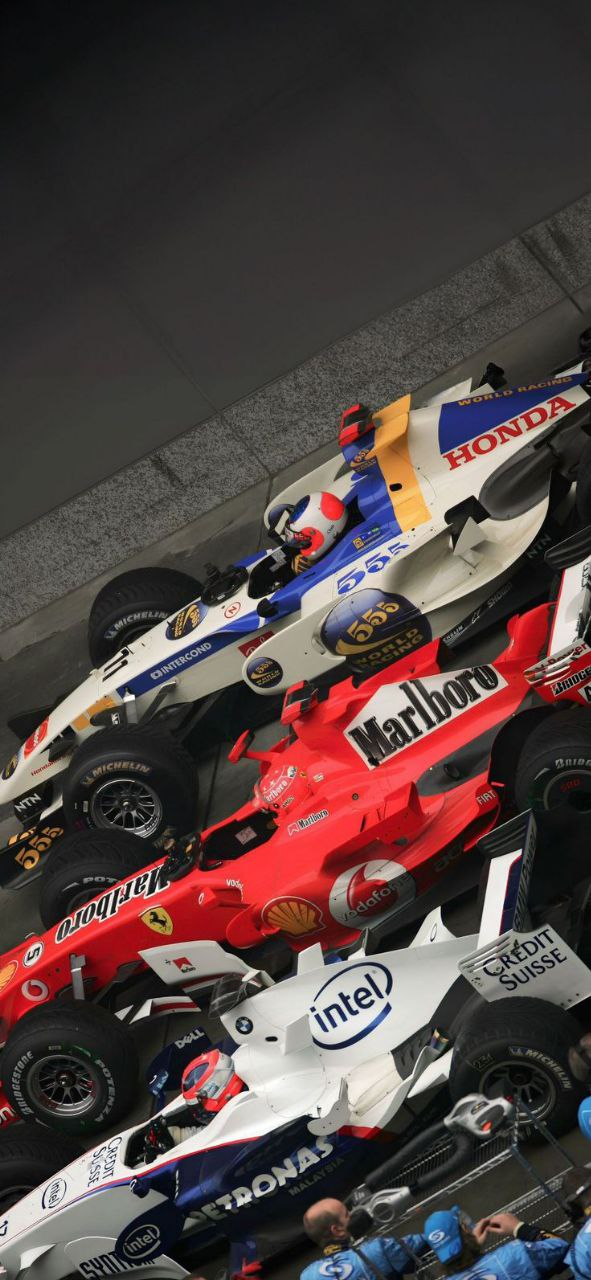
\includegraphics[width=1.0\paperwidth, height=\paperheight]{../img/fondo.jpg}} % Reducimos el ancho
}



\begin{document}


\newpage

	
	\title{Análisis para la Predicción de Tiempo de Vuelta usando Regresión Lineal Múltiple}
	\author{}
	\date{}
	\maketitle
	
	\section{Introducción}
	
	Melbourne (Gran Premio de Australia) es un circuito urbano ubicado en Albert Park, Melbourne. Con una longitud de 5303 metros, se caracteriza por ser una pista mixta que combina secciones de alta velocidad con curvas técnicas. Aunque es un circuito que se corre en sentido horario, las zonas más difíciles son aquellas con múltiples cambios de dirección, lo que exige un alto nivel de control y precisión.
	
	El clima en Melbourne es impredecible, con cambios repentinos de temperatura y posibles lluvias que complican las estrategias de los equipos. Las curvas de alta velocidad y las rectas relativamente cortas hacen que las paradas en boxes sean cruciales para los pilotos. Por lo tanto, es esencial tener un buen manejo de los neumáticos, especialmente en las zonas donde el asfalto es más abrasivo. El desempeño en la frenada y las aceleraciones de las curvas 1 y 3 son clave para conseguir tiempos rápidos.
	
	\begin{figure}[h]
		\centering
		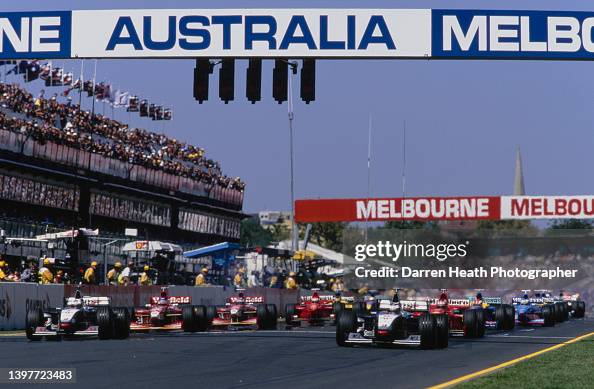
\includegraphics[width=0.8\textwidth]{../img/melbourne.jpg}
		\caption{Circuito de Melbourne, Gran Premio de Australia}
		\label{fig:melbourne}
	\end{figure}
	





\end{document}
